\documentclass[main.tex]{subfiles}
\begin{document}

\chapter{Joint Distributions and Transformations}\label{ch:ortak}

In statistics we rarely make do with a single random variable: a sample consists of $n$ random variables, estimators are functions of them, and a regression model describes the joint behaviour of several variables. This chapter systematises tools that were used implicitly in the previous chapters: random vectors and joint distributions\index{joint distribution@joint distribution}, the density criterion for independence, the distribution of sums (convolution\index{convolution@convolution}), the multivariate change of variables (Jacobian\index{jacobian method@Jacobian method}), the multivariate normal\index{multivariate normal distribution@multivariate normal distribution} distribution and order statistics\index{order statistics@order statistics}. These results explain where sampling distributions such as $\chi^2$, $t$, Beta and Gamma come from, and they form the basis of the normal sampling theory in Chapter~\ref{ch:guven}.

\section{Definitions}

\begin{definition}[Random Vector and Joint CDF]\index{joint distribution@joint distribution|textbf}
A function $\X=(X_1,\dots,X_k)^\top:\Omega\to\R^k$ whose components are random variables is called a \emph{random vector}. Its joint CDF is
\[
F_{\X}(x_1,\dots,x_k)=\P(X_1\le x_1,\dots,X_k\le x_k).
\]
A function $f_{\X}\ge0$ is called a \emph{joint density} if $\P(\X\in B)=\int_Bf_{\X}(\x)\,d\x$ for every Borel set $B\subseteq\R^k$; in the discrete case the joint pmf is $p_{\X}(\x)=\P(\X=\x)$.
\end{definition}

\begin{definition}[Marginal and Conditional Distributions]\index{marginal distribution@marginal distribution|textbf}
If $(X,Y)$ has joint density $f_{X,Y}$, the \emph{marginal} density of $X$ is $f_X(x)=\int f_{X,Y}(x,y)\,dy$. For $f_X(x)>0$, the \emph{conditional} density of $Y$ given $X=x$ is
\[
f_{Y\mid X}(y\mid x)=\frac{f_{X,Y}(x,y)}{f_X(x)} .
\]
This gives the \emph{product rule} $f_{X,Y}(x,y)=f_X(x)f_{Y\mid X}(y\mid x)$, the density form of hierarchical models and of Bayes' formula\index{bayes formula@Bayes' formula} (Chapter~\ref{ch:bayes}).
\end{definition}

\begin{definition}[Independence of Random Variables]\label{def:rd-bagimsiz}
$X_1,\dots,X_k$ are \emph{(mutually) independent} if
\[
\P(X_1\in B_1,\dots,X_k\in B_k)=\prod_{j=1}^k\P(X_j\in B_j)
\]
for all $B_1,\dots,B_k\in\B(\R)$. Equivalently, the joint CDF is the product of the marginal CDFs: $F_{\X}(\x)=\prod_jF_{X_j}(x_j)$ for every $\x$.
\end{definition}

\begin{definition}[Mean Vector and Covariance Matrix]\index{covariance@covariance|textbf}
$\bm\mu=\E\X=(\E X_1,\dots,\E X_k)^\top$ and
\[
\Sigma=\Cov(\X)=\E\big[(\X-\bm\mu)(\X-\bm\mu)^\top\big],\qquad\Sigma_{jl}=\Cov(X_j,X_l).
\]
\end{definition}

\begin{definition}[Multivariate Normal Distribution]\label{def:mvn}
$\X$ is called \emph{multivariate normal\index{multivariate normal distribution@multivariate normal distribution}}, written $\X\sim\Normal_k(\bm\mu,\Sigma)$, if $\mathbf a^\top\X$ is (univariate) normal for every $\mathbf a\in\R^k$ (constants, with variance $0$, included). If $\Sigma$ is positive definite, the density is
\[
f(\x)=(2\pi)^{-k/2}\det(\Sigma)^{-1/2}\exp\Big\{-\tfrac12(\x-\bm\mu)^\top\Sigma^{-1}(\x-\bm\mu)\Big\}.
\]
\end{definition}

\begin{definition}[Order Statistics]
The values $X_1,\dots,X_n$ arranged in increasing order, $X_{(1)}\le X_{(2)}\le\dots\le X_{(n)}$, are called the \emph{order statistics\index{order statistics@order statistics}}. $X_{(1)}$ is the minimum, $X_{(n)}$ the maximum, and $R=X_{(n)}-X_{(1)}$ the range.
\end{definition}

\section{Main Theorems and Proofs}

\begin{theorem}[Density Criterion for Independence]\label{thm:bagimsiz-carpan}
Let $(X,Y)$ have joint density\index{joint distribution@joint distribution} $f_{X,Y}$. Then $X\indep Y$ $\iff$ there exist non-negative functions $g,h$ such that $f_{X,Y}(x,y)=g(x)h(y)$ for almost every $(x,y)$.
\end{theorem}
\begin{proof}
($\Rightarrow$) Independence gives $F_{X,Y}=F_XF_Y$; taking the mixed derivative yields $f_{X,Y}=f_Xf_Y$.
($\Leftarrow$) Let $c_g=\int g$ and $c_h=\int h$; then $1=\iint gh=c_gc_h$. Since the marginals\index{marginal distribution@marginal distribution} are $f_X=c_hg$ and $f_Y=c_gh$, we get $f_Xf_Y=c_gc_h\,gh=f_{X,Y}$; as the densities factorise, so do the probabilities.
\end{proof}

\begin{remark}
The factorisation\index{factorisation theorem@factorisation theorem} criterion also involves the \emph{support}: although $f(x,y)=2\,\I\{0<x<y<1\}$ looks formally ``constant'', the factor $\I\{x<y\}$ cannot be written in the form $g(x)h(y)$; $X$ and $Y$ are dependent.
\end{remark}

\begin{theorem}[Convolution Formula]\label{thm:konvolusyon}\index{convolution@convolution}
If $X\indep Y$ with densities $f_X,f_Y$, the density of $Z=X+Y$ is
\[
f_Z(z)=\int_{-\infty}^\infty f_X(x)\,f_Y(z-x)\,dx=(f_X*f_Y)(z).
\]
In the discrete case, $p_Z(z)=\sum_xp_X(x)p_Y(z-x)$.
\end{theorem}
\begin{proof}
$F_Z(z)=\iint_{x+y\le z}f_X(x)f_Y(y)\,dy\,dx=\int f_X(x)F_Y(z-x)\,dx$; differentiating with respect to $z$ (under the integral sign, by dominated convergence) gives the result.
\end{proof}

\begin{theorem}[Multivariate Change of Variables]\label{thm:jacobian}
Let $\X$ have density $f_{\X}$ supported on an open set $A\subseteq\R^k$. Let $\mathbf g:A\to B$ be one-to-one, onto and continuously differentiable, and let the Jacobian\index{jacobian method@Jacobian method} determinant of its inverse $\mathbf h=\mathbf g^{-1}$,
\[
J(\mathbf y)=\det\Big[\frac{\partial h_j(\mathbf y)}{\partial y_l}\Big]_{j,l=1}^k ,
\]
be non-zero on $B$. Then the density of $\mathbf Y=\mathbf g(\X)$ is
\[
f_{\mathbf Y}(\mathbf y)=f_{\X}\big(\mathbf h(\mathbf y)\big)\,|J(\mathbf y)|,\qquad\mathbf y\in B .
\]
\end{theorem}
\begin{proof}
For every Borel set $C\subseteq B$, the change-of-variables theorem for multiple integrals gives
\[
\P(\mathbf Y\in C)=\P(\X\in\mathbf h(C))=\int_{\mathbf h(C)}f_{\X}(\x)\,d\x=\int_Cf_{\X}(\mathbf h(\mathbf y))|J(\mathbf y)|\,d\mathbf y .
\]
Since this holds for every $C$, the integrand is the density of $\mathbf Y$. (The case $k=1$ is Theorem~\ref{thm:donusum}.)
\end{proof}

\begin{remark}[A Practical Recipe]
When the distribution of $m<k$ functions of $k$ variables is required, make the transformation one-to-one by adding $k-m$ ``auxiliary'' variables, apply Theorem~\ref{thm:jacobian}, and then integrate the auxiliary variables out. Example~\ref{ex:beta-gamma} is a typical application of this recipe.
\end{remark}

\begin{proposition}[Properties of the Covariance Matrix]\label{prop:kovaryans}\index{covariance@covariance}
\begin{enumerate}
  \item $\Sigma$ is symmetric and positive semi-definite: $\mathbf a^\top\Sigma\mathbf a=\Var(\mathbf a^\top\X)\ge0$ for every $\mathbf a$.
  \item For $A\in\R^{m\times k}$ and $\mathbf b\in\R^m$, $\E[A\X+\mathbf b]=A\bm\mu+\mathbf b$ and $\Cov(A\X+\mathbf b)=A\Sigma A^\top$.
  \item If $\Sigma$ is singular, $\X$ lies with probability 1 in a hyperplane of $\R^k$ (it has no joint density).
\end{enumerate}
\end{proposition}
\begin{proof}
(1) $\mathbf a^\top\Sigma\mathbf a=\E[(\mathbf a^\top(\X-\bm\mu))^2]$. (2) Linearity of expectation. (3) If $\Sigma\mathbf a=\mathbf 0$, then $\Var(\mathbf a^\top\X)=0$, i.e.\ $\mathbf a^\top\X=\mathbf a^\top\bm\mu$ a.s.
\end{proof}

\begin{theorem}[Properties of the Multivariate Normal]\label{thm:mvn}
Let $\X\sim\Normal_k(\bm\mu,\Sigma)$.
\begin{enumerate}
  \item \textbf{(Linear transformation)} $A\X+\mathbf b\sim\Normal_m(A\bm\mu+\mathbf b,\,A\Sigma A^\top)$. In particular, every marginal (sub-vector) is normal.
  \item \textbf{(Construction)} If $\Sigma=LL^\top$ (e.g.\ Cholesky) and $\mathbf Z\sim\Normal_k(\mathbf 0,I)$, then $\bm\mu+L\mathbf Z\sim\Normal_k(\bm\mu,\Sigma)$.
  \item \textbf{(Uncorrelated = independent)} For a partition $\X=(\X_1,\X_2)$, if $\Cov(\X_1,\X_2)=\mathbf 0$ then $\X_1\indep\X_2$.
  \item \textbf{(Conditional distribution)} If $\bm\mu=(\bm\mu_1,\bm\mu_2)$, $\Sigma=\begin{pmatrix}\Sigma_{11}&\Sigma_{12}\\\Sigma_{21}&\Sigma_{22}\end{pmatrix}$ and $\Sigma_{22}$ is invertible, then
  \[
  \X_1\mid\X_2=\x_2\ \sim\ \Normal\Big(\bm\mu_1+\Sigma_{12}\Sigma_{22}^{-1}(\x_2-\bm\mu_2),\ \ \Sigma_{11}-\Sigma_{12}\Sigma_{22}^{-1}\Sigma_{21}\Big).
  \]
  \item \textbf{(Quadratic form)} If $\Sigma$ is positive definite, $(\X-\bm\mu)^\top\Sigma^{-1}(\X-\bm\mu)\sim\chi^2_k$.
\end{enumerate}
\end{theorem}
\begin{proof}
(1) For every $\mathbf c\in\R^m$, $\mathbf c^\top(A\X+\mathbf b)=(A^\top\mathbf c)^\top\X+\mathbf c^\top\mathbf b$ is normal; the mean and covariance come from Proposition~\ref{prop:kovaryans}(2).
(2) From (1), since $\Cov(L\mathbf Z)=LL^\top=\Sigma$.
(3) Via the characteristic function\index{characteristic function@characteristic function}: the CF of $\Normal_k$ is $\exp\{i\mathbf t^\top\bm\mu-\frac12\mathbf t^\top\Sigma\mathbf t\}$ (because every $\mathbf t^\top\X$ is normal). When $\Sigma_{12}=\mathbf 0$, $\mathbf t^\top\Sigma\mathbf t=\mathbf t_1^\top\Sigma_{11}\mathbf t_1+\mathbf t_2^\top\Sigma_{22}\mathbf t_2$ and the CF factorises; uniqueness of the CF (Theorem~\ref{thm:teklik}) gives independence.
(4) Let $B=\Sigma_{12}\Sigma_{22}^{-1}$ and $\mathbf W=\X_1-B\X_2$. Then $\Cov(\mathbf W,\X_2)=\Sigma_{12}-B\Sigma_{22}=\mathbf 0$ and $(\mathbf W,\X_2)$ is jointly normal; by (3), $\mathbf W\indep\X_2$. Hence the distribution of $\X_1=\mathbf W+B\X_2$ given $\X_2=\x_2$ is that of $\mathbf W+B\x_2$: mean $\bm\mu_1-B\bm\mu_2+B\x_2$ and covariance $\Cov(\mathbf W)=\Sigma_{11}-B\Sigma_{21}$.
(5) With $\Sigma=LL^\top$, $\mathbf Z=L^{-1}(\X-\bm\mu)\sim\Normal_k(\mathbf 0,I)$ and the quadratic form is $\mathbf Z^\top\mathbf Z=\sum Z_j^2\sim\chi^2_k$.
\end{proof}

\begin{remark}[Regression Interpretation]
The conditional mean in (4) is a \emph{linear} function of $\x_2$, and the conditional covariance does not depend on $\x_2$. In the bivariate case $\E[Y\mid X=x]=\mu_Y+\rho\frac{\sigma_Y}{\sigma_X}(x-\mu_X)$ and $\Var(Y\mid X)=\sigma_Y^2(1-\rho^2)$: the mathematical source of linear regression and of ``regression to the mean'' (Galton). This shows that the best predictor of Corollary~\ref{cor:en-iyi-kestirici} is linear in the normal model.
\end{remark}

\begin{theorem}[Distribution of Order Statistics]\label{thm:sira}
Let $X_1,\dots,X_n\iid F$ with density $f$.
\begin{enumerate}
  \item $F_{X_{(n)}}(x)=F(x)^n$ and $F_{X_{(1)}}(x)=1-[1-F(x)]^n$.
  \item The density of $X_{(k)}$ is
  \[
  f_{X_{(k)}}(x)=\frac{n!}{(k-1)!\,(n-k)!}F(x)^{k-1}\big[1-F(x)\big]^{n-k}f(x).
  \]
  \item The joint density of $(X_{(1)},X_{(n)})$ is $n(n-1)\big[F(y)-F(x)\big]^{n-2}f(x)f(y)$ for $x<y$.
\end{enumerate}
\end{theorem}
\begin{proof}
(1) $\{X_{(n)}\le x\}=\bigcap_i\{X_i\le x\}$ and independence; for $X_{(1)}$ use the complement.
(2) Heuristic derivation: the event $X_{(k)}\in[x,x+dx]$ means that $k-1$ observations fall below $x$, one in $[x,x+dx]$ and $n-k$ above. The multinomial\index{multinomial distribution@multinomial distribution} probability is $\frac{n!}{(k-1)!1!(n-k)!}F^{k-1}(f\,dx)(1-F)^{n-k}$. (Rigorous proof: differentiate $\P(X_{(k)}\le x)=\sum_{j\ge k}\binom nj F^j(1-F)^{n-j}$; the terms telescope.)
(3) $\P(X_{(1)}>x,X_{(n)}\le y)=[F(y)-F(x)]^n$; take the mixed derivative of $F_{X_{(1)},X_{(n)}}(x,y)=F(y)^n-[F(y)-F(x)]^n$.
\end{proof}

\section{Worked Examples}

\begin{example}[A Sum of Exponentials Is Gamma]\label{ex:ustel-gamma}
If $X,Y\iid\text{Exp}(\lambda)$, then for $z>0$ Theorem~\ref{thm:konvolusyon} gives
\[
f_{X+Y}(z)=\int_0^z\lambda e^{-\lambda x}\lambda e^{-\lambda(z-x)}dx=\lambda^2ze^{-\lambda z},
\]
which is the $\text{Gamma}(2,\lambda)$ density. By induction $\sum_{i=1}^nX_i\sim\text{Gamma}(n,\lambda)$; the result $2\lambda\sum X_i\sim\chi^2_{2n}$ used in Chapters~\ref{ch:cramer-rao} and~\ref{ch:karlin-rubin} comes from here. Similar convolutions\index{convolution@convolution} show that a sum of independent Poissons is Poisson, a sum of independent normals is normal, and a sum of independent $\chi^2$'s is $\chi^2$ (the degrees of freedom add).
\end{example}

\begin{example}[The Gamma--Beta Relation]\label{ex:beta-gamma}
Let $X\sim\text{Gamma}(\alpha,1)$ and $Y\sim\text{Gamma}(\beta,1)$ be independent. The inverse of the transformation $U=X+Y$, $V=X/(X+Y)$ is $x=uv$, $y=u(1-v)$, with
\[
J=\det\begin{pmatrix}v & u\\ 1-v & -u\end{pmatrix}=-u .
\]
By Theorem~\ref{thm:jacobian}, for $u>0$, $0<v<1$,
\[
f_{U,V}(u,v)=\frac{(uv)^{\alpha-1}e^{-uv}\,(u(1-v))^{\beta-1}e^{-u(1-v)}}{\Gamma(\alpha)\Gamma(\beta)}\,u
=\underbrace{\frac{u^{\alpha+\beta-1}e^{-u}}{\Gamma(\alpha+\beta)}}_{\text{Gamma}(\alpha+\beta,1)}\cdot\underbrace{\frac{\Gamma(\alpha+\beta)}{\Gamma(\alpha)\Gamma(\beta)}v^{\alpha-1}(1-v)^{\beta-1}}_{\text{Beta}(\alpha,\beta)} .
\]
By Theorem~\ref{thm:bagimsiz-carpan}, $U\indep V$, $U\sim\text{Gamma}(\alpha+\beta,1)$ and $V\sim\text{Beta}(\alpha,\beta)$. This is the standard way of generating Beta variates from Gammas, and a direct check of the Basu\index{basu s theorem@Basu's theorem} exercise ($T\indep X_1/T$) in Chapter~\ref{ch:tamlik}.
\end{example}

\begin{example}[The Box--Muller Transformation \cite{box58}]\label{ex:box-muller}
Let $U_1,U_2\iid\text{Uniform}(0,1)$ and
\[
Z_1=\sqrt{-2\ln U_1}\cos(2\pi U_2),\qquad Z_2=\sqrt{-2\ln U_1}\sin(2\pi U_2).
\]
In polar coordinates, $S=R^2=Z_1^2+Z_2^2=-2\ln U_1\sim\text{Exp}(1/2)=\chi^2_2$ and the angle $\Theta=2\pi U_2\sim\text{Uniform}(0,2\pi)$ are independent: $f_{S,\Theta}(s,\vartheta)=\frac12e^{-s/2}\cdot\frac1{2\pi}$. The inverse map $s=z_1^2+z_2^2$, $\vartheta=\operatorname{atan2}(z_2,z_1)$ has Jacobian\index{jacobian method@Jacobian method} determinant $\big|\partial(s,\vartheta)/\partial(z_1,z_2)\big|=2$, so by Theorem~\ref{thm:jacobian}
\[
f_{Z_1,Z_2}(z_1,z_2)=\frac12e^{-(z_1^2+z_2^2)/2}\cdot\frac{1}{2\pi}\cdot2=\frac{1}{2\pi}e^{-(z_1^2+z_2^2)/2},
\]
i.e.\ $Z_1,Z_2\iid\Normal(0,1)$. (Whereas the inverse transform method\index{inverse transform method@inverse transform method} needs $\Phi^{-1}$ for the normal, Box--Muller\index{box muller transform@Box--Muller transform} uses only $\ln$, $\sqrt{\cdot}$ and trigonometric functions.)
\end{example}

\begin{example}[The Ratio of Two Normals Is Cauchy]\label{ex:oran-cauchy}
Let $Z_1,Z_2\iid\Normal(0,1)$ and $W=Z_1/Z_2$. With the auxiliary variable $V=Z_2$ we have $z_1=wv$, $z_2=v$, $|J|=|v|$:
\[
f_W(w)=\int_{-\infty}^\infty\frac{1}{2\pi}e^{-v^2(1+w^2)/2}|v|\,dv=\frac{1}{\pi}\int_0^\infty ve^{-v^2(1+w^2)/2}dv=\frac{1}{\pi(1+w^2)} .
\]
The standard Cauchy is also the $t_1$ distribution ($Z_1/\sqrt{Z_2^2}$, by symmetry). The distribution that we saw in Example~\ref{ex:cauchy-beklenen} has no mean arises as the ratio of the two most ``well-behaved'' distributions.
\end{example}

\begin{example}[Uniform Order Statistics Are Beta]\label{ex:uniform-sira}
For $U_i\iid\text{Uniform}(0,1)$, Theorem~\ref{thm:sira}(2) gives $f_{U_{(k)}}(u)=\frac{n!}{(k-1)!(n-k)!}u^{k-1}(1-u)^{n-k}$, i.e.\ $U_{(k)}\sim\text{Beta}(k,n-k+1)$ and $\E U_{(k)}=\frac{k}{n+1}$. By the probability integral transform\index{probability integral transform@probability integral transform} (Theorem~\ref{thm:pit}), $F(X_{(k)})\sim\text{Beta}(k,n-k+1)$ for any continuous $F$: this is the source of quantile confidence intervals and of the plotting positions $k/(n+1)$ in Q--Q plots. For the range, Theorem~\ref{thm:sira}(3) gives $R=U_{(n)}-U_{(1)}\sim\text{Beta}(n-1,2)$.
\end{example}

\begin{example}[A Vector with Normal Marginals That Is Not Jointly Normal]\label{ex:normal-degil}
Let $X\sim\Normal(0,1)$ and let $S$, independent of $X$, take the values $+1$ and $-1$ with equal probability ($\frac12$); set $Y=SX$. By symmetry $Y\sim\Normal(0,1)$, and $\Cov(X,Y)=\E[S]\E[X^2]=0$. However, since $|Y|=|X|$, $X$ and $Y$ are not independent; moreover, $X+Y$ is exactly $0$ with probability $\frac12$, so it is not normal. ``Uncorrelated = independent'' in Theorem~\ref{thm:mvn}(3) holds only under \emph{joint} normality; normal marginals\index{marginal distribution@marginal distribution} are not enough.
\end{example}

\begin{example}[Bivariate Normal: Height and Weight]
For height $X$ (cm) and weight $Y$ (kg) let $\mu_X=170$, $\sigma_X=10$, $\mu_Y=70$, $\sigma_Y=12$, $\rho=0.6$. By Theorem~\ref{thm:mvn}(4),
\[
\E[Y\mid X=185]=70+0.6\cdot\frac{12}{10}(185-170)=80.8,\qquad\sqrt{\Var(Y\mid X)}=12\sqrt{1-0.36}=9.6 .
\]
The expected weight of a person of height 185 cm is only $0.9\sigma_Y$ above the mean, although the height is $1.5\sigma_X$ above its mean: regression to the mean.
\end{example}

\section{Computational Applications}

\subsection{Box--Muller and Gamma--Beta Independence}

\pycode{code/ch04/c04_1_box_muller_gamma_beta.py}
\begin{lstlisting}[style=output]
Box-Muller: mean=(-0.0006, -0.0021) | var=(1.0024, 1.0002) | Corr=-0.0022 | Corr(Z1^2,Z2^2)=-0.0038
KS p-value (Z1 ~ N(0,1)): 0.835
Gamma-Beta: Corr(U, V)=-0.0002 | Corr(U, V^2)=-0.0003
  E[V]=0.2857 (Beta mean 0.2857) | E[U]=7.0062 (Gamma mean 7.0)
  KS: V~Beta(2.0,5.0) p=0.498
  E[V] within slices of U: [0.2863 0.2853 0.2853 0.286 ]
\end{lstlisting}

\subsection{Multivariate Normal: Cholesky Generation, Conditional Distribution, Mahalanobis}

\pycode{code/ch04/c04_2_multivariate_normal_cholesky.py}
\begin{lstlisting}[style=output]
Sample covariance - Sigma (largest absolute difference): 0.149
E[X1|x2,x3]: theory=175.000, slice=174.834 | sd: theory=8.000, slice=8.123 (n=5292)
Mahalanobis D^2: mean=2.9988 (3) | P(D^2 > chi2_3,0.05)=0.0499 (0.05)
\end{lstlisting}

\subsection{Order Statistics and a Vector That Is Not Jointly Normal}

\pycode{code/ch04/c04_3_order_statistics_not_jointly_normal.py}
\begin{lstlisting}[style=output]
U_(1) : mean=0.1003 (k/(n+1)=0.1000) | KS p, Beta(1,9): 0.545
U_(3) : mean=0.2999 (k/(n+1)=0.3000) | KS p, Beta(3,7): 0.391
U_(5) : mean=0.4998 (k/(n+1)=0.5000) | KS p, Beta(5,5): 0.344
U_(9) : mean=0.9000 (k/(n+1)=0.9000) | KS p, Beta(9,1): 0.902
Range: mean=0.7997 (Beta(8,2) mean 0.8000)
Y=SX: Corr(X,Y)=+0.0120 | Corr(X^2,Y^2)=+1.0000 | P(X+Y=0)=0.491
\end{lstlisting}

\begin{figure}[h]
\centering
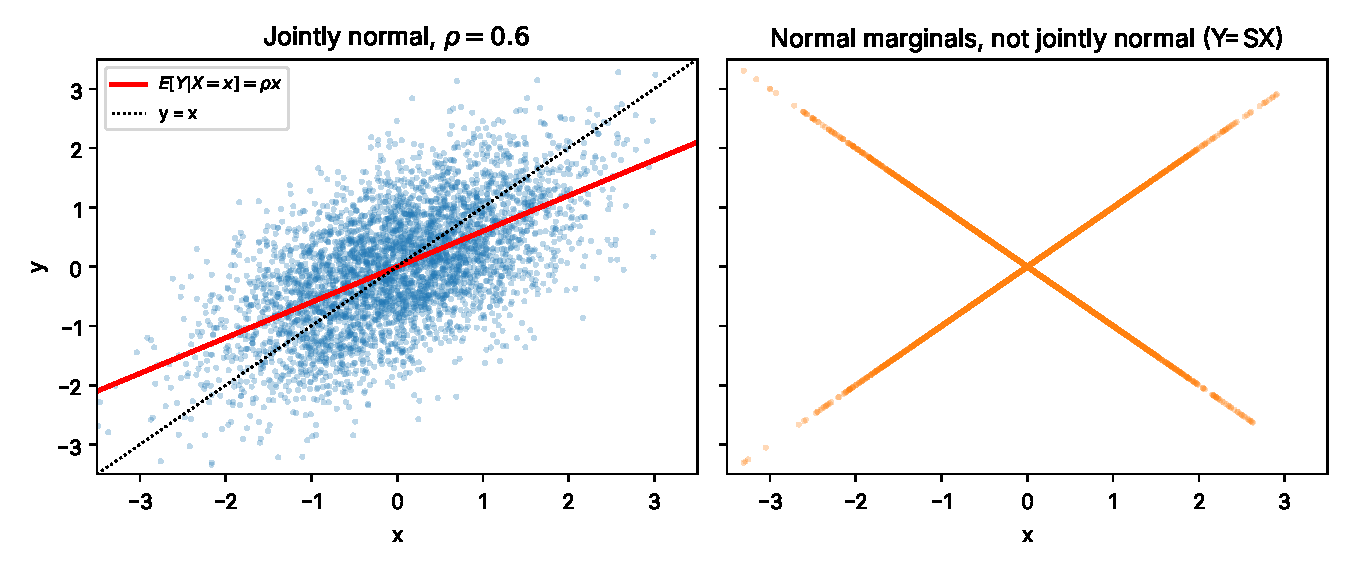
\includegraphics[width=0.9\textwidth]{figures/ortak_normal.pdf}
\caption{Left: a bivariate normal and the conditional mean line; since the slope is $\rho<1$, it is flatter than the line $y=x$ (regression to the mean). Right: $X$ and $Y=SX$ are each standard normal and uncorrelated, but their joint distribution concentrates on the two diagonals --- it is not jointly normal and the variables are dependent.}
\end{figure}

\section{Comments and Notes}

\begin{remark}[Copulas]
Sklar\index{sklar s theorem@Sklar's theorem}'s theorem \cite{sklar59}: every joint CDF\index{joint distribution@joint distribution} can be written as $F(\x)=C(F_1(x_1),\dots,F_k(x_k))$ with the marginal\index{marginal distribution@marginal distribution} CDFs and a \emph{copula\index{copula@copula}} $C:[0,1]^k\to[0,1]$; if the marginals are continuous, $C$ is unique. This way of separating the dependence structure from the marginals is widely used in financial risk and hydrology. Example~\ref{ex:normal-degil} shows that the same (normal) marginals can be combined through very different copulas.
\end{remark}

\begin{remark}[The Central Role of the Multivariate Normal]
Because of the multivariate CLT\index{central limit theorem clt@central limit theorem (CLT)} (Theorem~\ref{thm:cok-degiskenli-clt}), vectors of estimators are approximately multivariate normal\index{multivariate normal distribution@multivariate normal distribution} in large samples. That is why the properties in Theorem~\ref{thm:mvn} --- linear transformations, conditional distributions, the $\chi^2$ distribution of quadratic forms --- are used throughout Wald tests\index{wald test@Wald test} (Chapter~\ref{ch:lrt}), confidence ellipsoids and linear models.
\end{remark}

\begin{remark}[A Computational Note]
When generating multivariate normals, using the Cholesky factor $L$ instead of $\Sigma^{1/2}$ is both faster ($O(k^3/3)$) and numerically more stable. For conditional distributions and Mahalanobis distances, solving a linear system (\texttt{np.linalg.solve}) is preferable to forming $\Sigma^{-1}$ explicitly.
\end{remark}

% --- CHAPTER SUMMARY ---
\section{Chapter Summary}
\begin{summary}
\begin{itemize}
  \item The joint distribution determines the marginal and conditional distributions. With densities, independence is equivalent to factorisation of the joint density (Theorem~\ref{thm:bagimsiz-carpan}).
  \item The density of an independent sum is found by convolution (Theorem~\ref{thm:konvolusyon}), and that of a general one-to-one transformation by the Jacobian method (Theorem~\ref{thm:jacobian}). The Box--Muller transformation is an application of the latter.
  \item The covariance matrix is symmetric and positive semi-definite, and $\Cov(A\X)=A\Sigma A^\top$ (Proposition~\ref{prop:kovaryans}).
  \item The multivariate normal distribution is closed under linear transformations, and its marginal and conditional distributions are normal (Theorem~\ref{thm:mvn}). Under joint normality, uncorrelatedness is equivalent to independence; normal marginals do not imply joint normality.
  \item The distributions of order statistics can be written explicitly in terms of $F$ and $f$ (Theorem~\ref{thm:sira}). These results underlie the distribution-free intervals of Chapter~\ref{ch:parametrik-olmayan}.
\end{itemize}
\end{summary}
% --- END OF CHAPTER SUMMARY ---

\paragraph{Further reading.} \cite[Chapter~4]{casella}, \cite[Chapters~2--3]{wasserman}; for the multivariate normal\index{multivariate normal distribution@multivariate normal distribution} see \cite[Chapters~2--3]{seber}.

\section{Exercises}

\begin{exercise}\label{exr:04-1}
For $X,Y\iid\text{Uniform}(0,1)$, find the density of $X+Y$ (the triangular distribution) by convolution. Write down the mean and variance of the sum of $n$ independent uniforms (Irwin--Hall), and explain why for $n=12$, $\sum U_i-6$ was once used as an ``approximately normal'' generator.
\hfill\hyperref[coz:04-1]{\footnotesize$\rightarrow$\,Solution}
\end{exercise}

\begin{exercise}\label{exr:04-2}
Let $Z\sim\Normal(0,1)$ and $V\sim\chi^2_k$ be independent. Derive the density of $T=Z/\sqrt{V/k}$ using Theorem~\ref{thm:jacobian} (auxiliary variable $V$) and obtain the $t_k$ density.
\hfill\hyperref[coz:04-2]{\footnotesize$\rightarrow$\,Solution}
\end{exercise}

\begin{exercise}\label{exr:04-3}
For $X_i\iid\text{Exp}(\lambda)$, show that $X_{(1)}\sim\text{Exp}(n\lambda)$ and that the ``spacings'' $D_k=(n-k+1)(X_{(k)}-X_{(k-1)})$ are i.i.d.\ $\text{Exp}(\lambda)$ (Rényi's representation). Verify this by simulation.
\hfill\hyperref[coz:04-3]{\footnotesize$\rightarrow$\,Solution}
\end{exercise}

\begin{exercise}\label{exr:04-4}
For $(X,Y)\sim\Normal_2$ ($\mu=0$, $\sigma=1$, correlation $\rho$), show that $\P(X>0,Y>0)=\frac14+\frac{\arcsin\rho}{2\pi}$ (Sheppard's formula). Hint: polar coordinates and Theorem~\ref{thm:mvn}(2).
\hfill\hyperref[coz:04-4]{\footnotesize$\rightarrow$\,Solution}
\end{exercise}

\chapterlinks{04}

\end{document}
